\documentclass{theozettel}

%%%%%%%%%%%%%%%%%%%%%%%%%%%%%%%%%%%%%%%%%%%%%%%%%%%%%%%%%%%%%%%%%%%%%%%%%%%%%%%%%%%%%%%%%%%%%%%%%%%%%%%%%%%%%%
% page geometry
%%%%%%%%%%%%%%%%%%%%%%%%%%%%%%%%%%%%%%%%%%%%%%%%%%%%%%%%%%%%%%%%%%%%%%%%%%%%%%%%%%%%%%%%%%%%%%%%%%%%%%%%%%%%%%
\geometry{
	left=20mm,
	right=20mm,
	top=25mm,
	bottom=20mm
}
%%%%%%%%%%%%%%%%%%%%%%%%%%%%%%%%%%%%%%%%%%%%%%%%%%%%%%%%%%%%%%%%%%%%%%%%%%%%%%%%%%%%%%%%%%%%%%%%%%%%%%%%%%%%%%

\pgfplotsset{compat=1.16}

%\renewcommand{\phi}{\varphi}

\usepackage{parskip}
\usepackage{dsfont}
\newcommand{\difd}{\text{d}}
\usepackage{titlesec} 
\titleformat{\section}[runin]
{\normalfont\large\bfseries}{\thesubsection}{1em}{}
\titleformat{\subsection}[runin]
  {\normalfont\normalsize\bfseries}{\thesubsubsection}{1em}{}
  
\renewcommand{\epsilon}{\varepsilon}
\newcommand{\vol}{\operatorname{vol}}

\theoI{8}

\begin{document}
\punkteIII{9.1}{9.3}{9.5}

\section*{Aufgabe 9.1} 

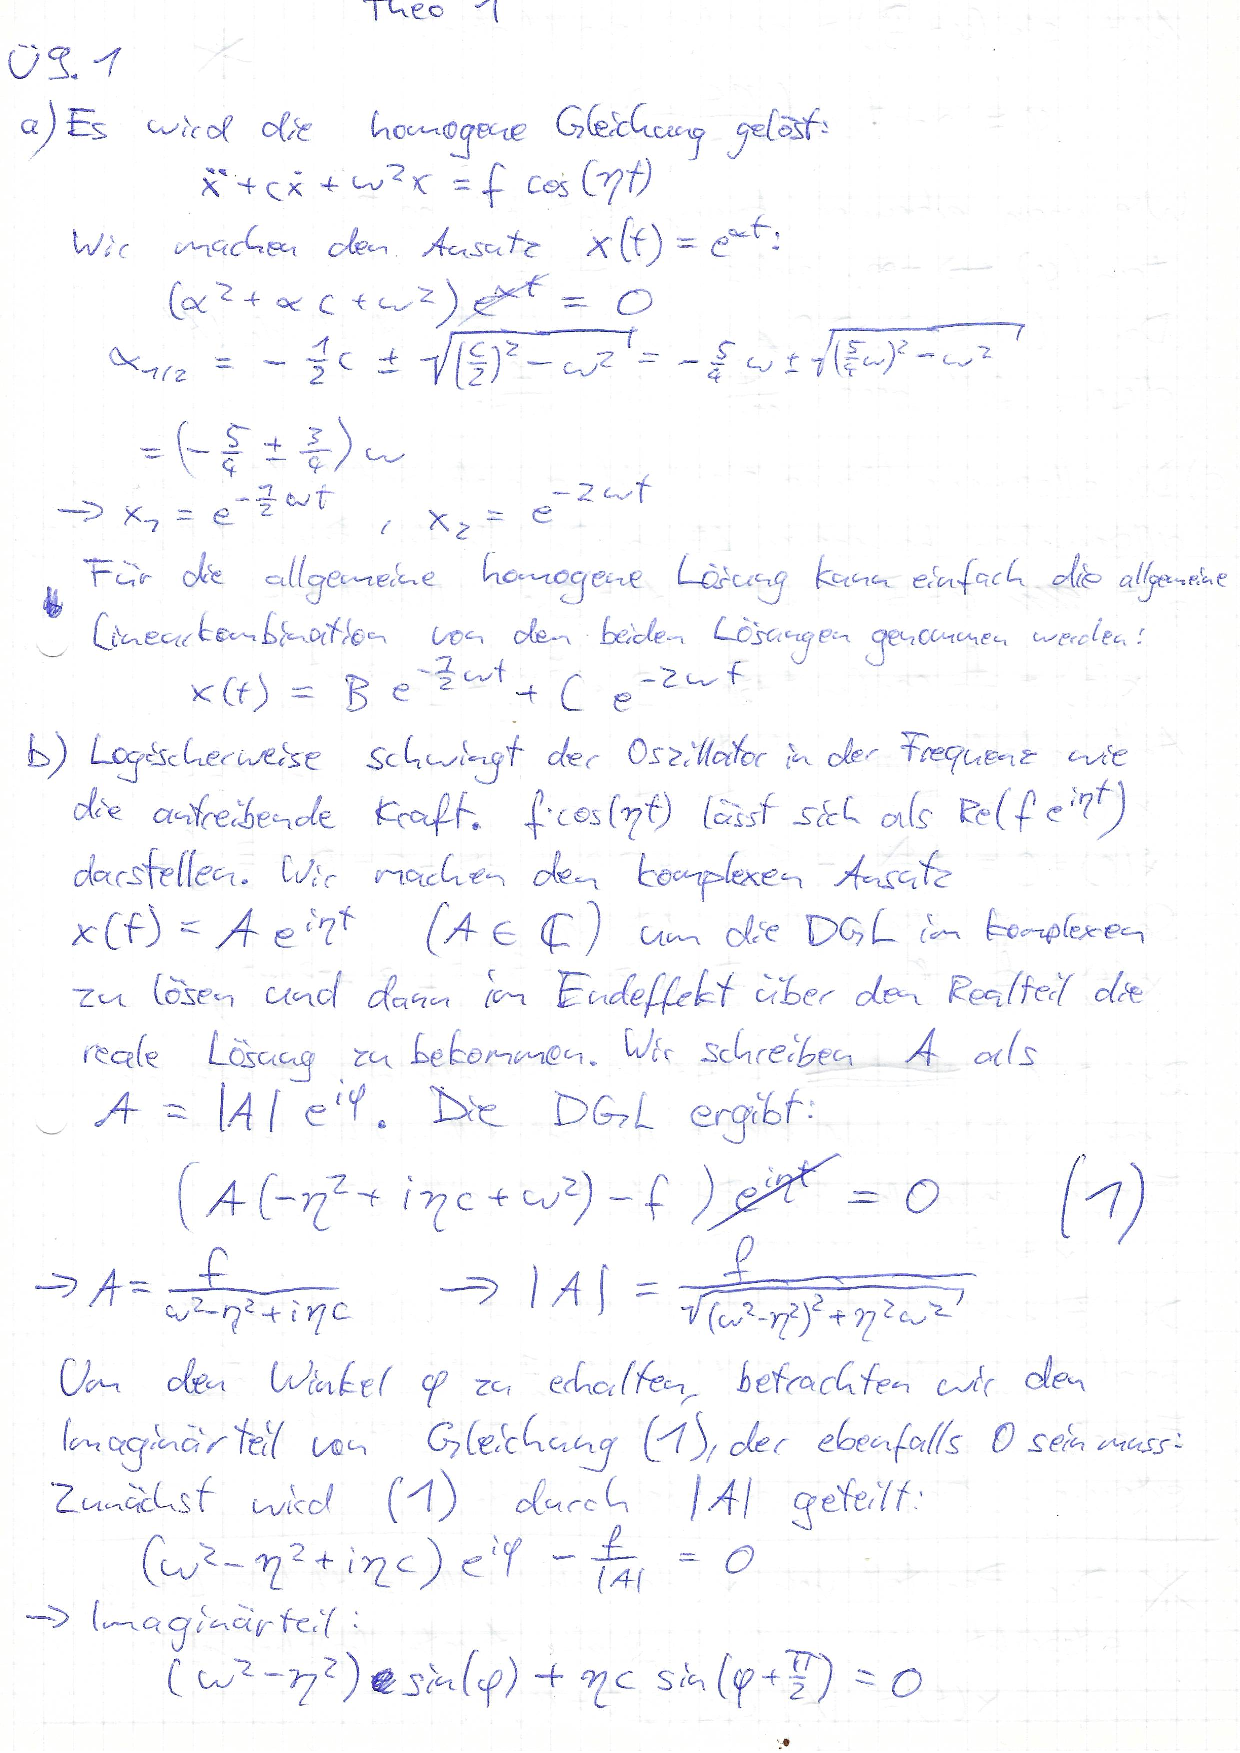
\includepdf[pages=-]{Theo1U9A1.pdf}



\section*{Aufgabe 9.3}
Wir wählen einen Punkt $P$ der Erdoberfläche bei Breitengrad $\varphi$ und lokal ein Koordinatensystem, mit Basisvektoren in Richtung Osten $O$, Norden $N$ und radial vom Erdmittelpunkt weg $H$.
	\begin{figure}[H]
	\centering
	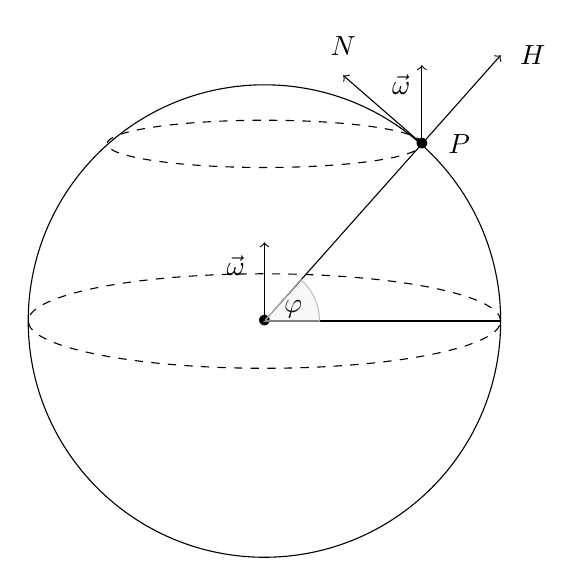
\begin{tikzpicture}
		\draw(0,0) circle (3cm);
  		\draw [rotate around={0.:(0.,0.)},dash pattern=on 3pt off 3pt] (0,0) ellipse (3cm and 0.6cm);
  		\draw [rotate around={0.:(0.,0.)},dash pattern=on 3pt off 3pt] (0,2.25) ellipse (2cm and 0.3cm);
  		\node at (0,0)  {$\bullet$};
  		\draw (0,0) -- (2, 2.25);
  		\node at (2,2.25) [label=right:$P$] {$\bullet$};
  		
  		\draw [->] (2,2.25) -- (3,3.375);
  		\node at (3,3.375) [label=right:$H$] {};
  		
  		\draw [->] (2,2.25) -- (1,3.12);
  		\node at (1,3.12) [label=above:$N$] {};
  		
  		\draw (0,0) -- (3,0);
  		\node at (0,0.15) [label=right:$\varphi$] {};
  		\draw [shift={(0,0)}, lightgray, fill, fill opacity=0.1] (0,0) -- (0.:0.7) arc (0.:49.:0.7) -- cycle;
  		
  		\draw [->] (0,0) -- (0,1);
  		\node at (0,0.7) [label=left:$\vec{\omega}$] {};
  		
  		\draw [->] (2,2.25) -- (2,3.25);
  		\node at (2.1,3) [label=left:$\vec{\omega}$] {};
	\end{tikzpicture}
	\end{figure}

Sei $R$ der Radius der Erde. Geometrisch sehen wir sofort (im Koordinatensystem der Erde) $P_{0} = R(0, \cos(\phi), \sin(\phi))$. Wir nehmen zunächst an $\vec{\omega} = 0$. Dann entspricht die Bewegung vom zu $P$ gehörenden Koordinatensystem der Bewegung auf der Kreisbahn um die Erde auf Höhe des Winkels $\phi$ um den Radius $(P_{0})^{2}$. Eine ganze Umdrehung entspricht genau $24 h$. Für einen Massepunkt in $\vec{r}_{0}$ zum Zeitpunkt $t = 0$ erhalten wir also im Fall $\vec{\omega} = 0$, dass für $\lambda = \frac{2\pi}{24h}$ gilt \[\vec{r}_{0}(t) = \vec{r}_{0} + (R\cos(\phi)\sin(\lambda t),\ R\cos(\phi)\cos(\lambda t), \ R\sin(\phi)  ).\]
Nun nehmen wir $\vec{\omega} \neq 0$ an, also drehe sich die Erde um die $x_{3}$-Achse, sodass eine vollständige Drehung genau einem Tag entspreche. Diese Drehung entspricht genau der linearen Abbildung (linear zum festen Zeitpunkt $t$) mit $(0,0,1) \mapsto = (0,0,1)$, $(1,0,0) \mapsto (\cos(\lambda t),\sin(\lambda t), 0)$ und $(0,1,0) \mapsto (-\sin(\lambda t), \cos(\lambda t), 0)$, also mit der Darstellungsmatrix \[R = R\mqty(\cos(\lambda t) & -\sin(\lambda t) & 0 \\ \sin(\lambda t) & \cos(\lambda t) & 0 \\ 0 & 0 & 1)\] wie wir an folgender Skizze geometrisch sehen (für $(1,0,0)$):
	\begin{figure}[H]
	\centering
	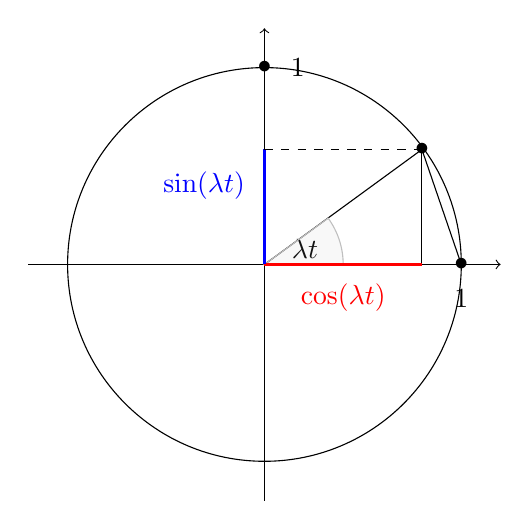
\begin{tikzpicture}
		\draw [->] (-3,0) -- (3,0);
		\node at (2.5,0) [label=below:$1$] {$\bullet$};
		
		\draw [->] (0,-3) -- (0,3);
		\node at (0,2.5) [label=right:$1$] {$\bullet$};
		
		\draw(0,0) circle (2.5cm);
		
		\node at (2,1.46) {$\bullet$};
		\draw (2,1.46) -- (2.5,0);
		\draw (2,1.46) -- (0,0);
		\draw (2,1.46) -- (2,0);
  		\node at (0.1,0.2) [label=right:$\lambda t$] {};
  		\draw [shift={(0,0)}, lightgray, fill, fill opacity=0.1] (0,0) -- (0.:1.) arc (0.:36.:1.) -- cycle;
  		\draw [red,thick] (0,0) -- (2,0);
  		\node at (1,0) [label=below:$\textcolor{red}{\cos(\lambda t)}$] {};
  		\draw [blue,thick] (0,0) -- (0,1.46);
  		\node at (0,1) [label=left:$\textcolor{blue}{\sin(\lambda t)}$] {};
  		\draw [dash pattern=on 3pt off 3pt] (0,1.46) -- (2,1.46);
	\end{tikzpicture}
	\end{figure}
Ferner gilt $\dot{R}(0) = \mqty(0 & -\lambda & 0 \\ \lambda & 0 & 0 \\0 & 0 &0)$. Also erhalten wir (im Koordinatensystem der Erde) $\vec{\omega} = (0,0,\lambda)$ mit $\omega = \lambda$ und erhalten geometrisch aus der ersten Skizze im lokalen Koordinatensystem: $\vec{\omega} = \omega (0, \cos(\phi), \sin(\phi))$. 


	%\[
%		\vec{r}(t) = \vec{r}_{0}(t) + R(t) \cdot \vec{y}(t)
	%\]
%Wobei $\vec{y}$ die Trajektorie des Massepunkts im Koordinatensystem der Erde ist. Wir erhalten: 
	%\[
	%	RF = \ddot{\vec{r}} = \ddot{\vec{r}}_{0} + (R \cdot \vec{y})^{\dot{•}}.
	%\]
%Wir erhalten $\vec{y}$, wenn wir alle Terme in $\dot{\vec{\omega}}$ und quadratisch in $\omega$ vernachlässigen durch:
	%\[
	%	\ddot{\vec{y}} = \frac{F}{m} - [R^{-1}\ddot{\vec{r}}_{0} + 2\vec{\omega} \times \ddot{\vec{y}}].
	%\]


%Auf einen Massepunkt im Punkt $\vec{r}_{0} = (0,r_{2},r_{3})$ wirkt die Gravitationskraft mit $F = (0, -g\cos(\varphi), -g\sin(\varphi))$. Wir erhalten die Bewegungsgleichung, wenn wir alle Terme in $\dot{\vec{\omega}}$ und quadratisch in $\omega$ vernachlässigen:
	%\begin{align*}
	%	m\ddot{r}(t) = F - m [
	%\end{align*}



\section*{Aufgabe 9.5} 
Die Voraussetzung der Differenzierbarkit für l'Hospital ist hier stets gegeben.
\begin{enumerate}[(i)]
	\item 	Die Regel von l'Hospital liefert wegen $\sin(x) \stackrel{x \to 0}{\longrightarrow} 0$ und $x \stackrel{x \to 0}{\longrightarrow} 0$:
			\[
				\lim_{x \to 0} \frac{\sin(x)}{x} = \lim_{x \to 0} \frac{\cos(x)}{1} = 1.
			\]
			
	\item 	Die Regel von ä'Hospital liefert wegen $\frac{1}{x} \stackrel{x \to 0}{\longrightarrow} \infty$ und $\log(x) \stackrel{x \to 0}{\longrightarrow} \infty$:
			\[
				\lim_{x \to 0} \frac{\log(x)}{\frac{1}{x}} = \lim_{x \to 0} \frac{\frac{1}{x} }{ \frac{-1}{x^{2}}} = \lim_{x \to 0} -x = 0.
			\]
	
	\item 	Wir verwenden, dass aus Ana bekannt ist, dass $\lim_{x \to \infty} \qty(1 - \frac{z}{x})^{x} = e^{-z}$. Da Produkt zweier konvergenter Folge gegen das Produkt der Grenzwerte konvergiert folgt:
			\[
				\lim_{x \to \infty} \qty(1-\frac{2}{x})^{5x} = \left( \lim_{x \to \infty} \qty(1-\frac{2}{x})^{x} \right)^{5} = \qty(e^{-2})^{5} =\frac{1}{e^{10}}.
			\]
	
	\item 	Die Regel von l'Hospital liefert wegen $\cos(x) - \sqrt{1-x^{2}} \stackrel{x \to 0}{\longrightarrow} 0$ und $x^{4} \stackrel{x \to 0}{\longrightarrow} 0$ (bei $(*)$ gilt wieder der $0/0$ Fall)
			\begin{align*}
				\lim_{x \to 0} \frac{\cos(x) - \sqrt{1-x^{2}}}{x^{4}} &= \lim_{x \to 0} \frac{-\sin(x) - \frac{x}{\sqrt{1-x^{2}}}}{4x^{3}} \\
				&\stackrel{(*)}{=} \lim_{x \to 0} \frac{-\cos(x) + \frac{1}{(1-x^{2})^{\frac{3}{2}}}}{12x^{2}}  \\
				&\stackrel{(*)}{=} \lim_{x \to 0} \frac{\sin(x) + \frac{3x}{(1-x^{2})^{\frac{5}{2}}}}{24x^{1}} \\
				&\stackrel{(*)}{=} \lim_{x \to 0} \frac{\cos(x) + \frac{3(4x^2 + 1)}{(1-x^{2})^{\frac{7}{2}}}}{24} = \frac{1 + 3}{24} = \frac{1}{6}.			
			\end{align*}
	
	\item 	Wir zeigen dass $\lim_{x \to 0^{+}} \frac{1}{\frac{\cot(x)}{\log(x)}} = 0$. Daraus folgt dass $\lim_{x \to 0^{+}} \frac{\cot(x)}{\log(x)} = \infty$. Die Regel von l'Hospital für $\cot(x) \stackrel{x \to 0^{+}}{\longrightarrow} \infty$ und $\log(x)\stackrel{x \to 0^{+}}{\longrightarrow} \infty$ liefert:
			\begin{align*}
				\lim_{x \to 0^{+}} \frac{\log(x)}{\cot(x)} &= \lim_{x \to 0^{+}} \frac{\frac{1}{x}}{-\frac{1}{\sin^{2}(x)}}  = \lim_{x \to 0^{+}} \frac{\sin^{2}(x)}{-x} \\
				&\stackrel{0/0}{=} \lim_{x \to 0^{+}} \frac{2\cos(x)\sin(x)}{-1} = 0.
			\end{align*}
	
	\item 	Die Regel von l'Hospital für $\sinh^{2}(x)\stackrel{x \to 0}{\longrightarrow} 0$ und $ x\sin(2x) \stackrel{x \to 0}{\longrightarrow} 0$ sowie wiederholtes Anwenden der Regel liefern:
			\begin{align*}
				\lim_{x \to 0} \frac{x\sin(2x)}{\sinh^{2}(x)} &= \lim_{x \to 0} \frac{\sin(2x) + 2x\cos(2x)}{2\sinh(x)\cosh(x)} \\
				&= \lim_{x \to 0} \frac{2\cos(2x) + 2 \cos(2x) + 4x\sin(2x)}{2(\sinh^{2}(x) + \cosh^{2}(x))} = \frac{2+2+0}{2(0+1)} = 2.
			\end{align*}
\end{enumerate}



\end{document}
